\documentclass[12pt,a4paper]{article}

%Define a test for doing PDF format -- use different code below
\newif\ifPDF
\ifx\pdfoutput\undefined\PDFfalse 
\else\ifnum\pdfoutput > 0\PDFtrue 
     \else\PDFfalse 
     \fi 
\fi

\textwidth=161 mm
\textheight=240 mm
\topmargin=-18 mm
\oddsidemargin=0 mm
\parindent=6 mm

\usepackage[sort]{natbib}
\usepackage{lscape}
\bibpunct[,]{(}{)}{;}{a}{}{,}

\newcommand{\eg}{e.g.\ }
\newcommand{\ie}{i.e.\ }
\newcommand{\hi}{H{\sc i}}
\newcommand{\hipass}{{\sc hipass}}
\newcommand{\progname}{{\tt Duchamp}}
\newcommand{\diff}{{\rm d}}
\newcommand{\entrylabel}[1]{\mbox{\textsf{\bf{#1:}}}\hfil}
\newenvironment{entry}
        {\begin{list}{}%
                {\renewcommand{\makelabel}{\entrylabel}%
                        \setlength{\labelwidth}{30mm}%
                        \setlength{\labelsep}{5pt}%
                        \setlength{\itemsep}{2pt}%
                        \setlength{\parsep}{2pt}%
                        \setlength{\leftmargin}{35mm}%
                }%
        }%
{\end{list}}


\title{A Guide to the {\it Duchamp} Source Finding Software}
\author{Matthew Whiting\\
%{\small \href{mailto:Matthew.Whiting@csiro.au}{Matthew.Whiting@csiro.au}}\\
Australia Telescope National Facility\\CSIRO}
%\date{January 2006}
\date{}

% If we are creating a PDF, use different options for graphicx, hyperref.
\ifPDF
  \usepackage[pdftex]{graphicx,color}
  \usepackage[pdftex]{hyperref}
  \hypersetup{colorlinks=true,% 	    
            % citecolor=black,%
            % filecolor=black,%
            % linkcolor=black,%
            % urlcolor=black,%
	      }
\else
  \usepackage[dvips]{graphicx} 
  \usepackage[dvips]{hyperref} 
\fi

\begin{document}

\maketitle
\tableofcontents

\newpage
\section{Introduction and getting going quickly}

This document gives details on the use of the program Duchamp. This
has been written to provide a source-detection facility for
spectral-line data cubes. The basic execution of Duchamp is to read
in a FITS data cube, find sources in the cube, and produce a text
file of positions, velocities and fluxes of the detections, as well as
a postscript file of the spectra of each detection. 

So, you have a FITS cube, and you want to find the sources in it. What
do you do? The first step is to make an input file that contains the
list of parameters. Brief and detailed examples are shown in
Appendix~\ref{app-input}. This provides the input file name, the various
output files, and defines various parameters that control the
execution.

The program is run by the command
\begin{quote}
{\tt Duchamp -p [parameter file]}
\end{quote}
replacing {\tt [parameter file]} with the name of the file you have
just created/copied. The program will then work away and give you the
list of detections and their spectra. The program execution is
summarise below, and detailed in \S\ref{sec-flow}. Information on
inputs is in \S\ref{sec-param} and Appendix~\ref{app-param}, and
descriptions of the output is in \S\ref{sec-output}.

\subsection{A summary of the execution steps}

The basic flow of the program is summarised here. All these steps are
discussed in more detail in the following sections, so read on if
you have questions!
\begin{enumerate}
\item The parameter file given on the command line is read in, and the
  parameters absorbed.
\item From the parameter file, the FITS image is located and read in
  to memory.
\item If requested, blank pixels are trimmed from the edges, and
  channels corresponding to bright (\eg Galactic) emission are
  excised. 
\item If requested, the baseline of each spectrum is removed.
\item If the reconstruction method is requested, the cube is
  reconstructed using the {\it {\' a} trous} wavelet method.
\item Searching for objects then takes place, using the requested
  thresholding method.
\item The list of objects is trimmed by merging neighbouring objects
  and removing those deemed unacceptable.
\item The baselines and trimmed pixels are replaced prior to output.
\item The details on the detections are written to screen and to the
  requested output file.
\item Maps showing the spatial location of the detections are written.
\item The integrated spectra of each detection are written to a
  postscript file. 
\item If requested, the reconstructed array can be written to a new
  FITS file.
\end{enumerate}

\subsection{Guide to terminology}

First, a brief note on the use of terminology in this guide. Duchamp
is designed to work on FITS ``cubes''. These are FITS\footnote{FITS is
the Flexible Image Transport System -- see \citet{hanisch01} or
websites such as 
\href{http://fits.cv.nrao.edu/FITS.html}{http://fits.cv.nrao.edu/FITS.html}
for details.} image arrays with three dimensions -- they are assumed
to have the following form: the first two dimensions (referred to as
$x$ and $y$) are spatial directions (that is, relating to the position
on the sky), while the third dimension, $z$, is the spectral
direction, which can correspond to frequency, wavelength, or velocity.

Each spatial pixel (a given $(x,y)$ coordinate) can be said to be a
single spectrum, while a slice through the cube perpendicular to the
spectral direction at a given $z$-value is a single channel (the 2-D
image is a channel map).

Features that are detected are assumed to be positive. If one wants to
search for absorption (negative) features, try multiplying your cube
by $-1$ before running Duchamp.

Note that it is possible to run Duchamp on a two-dimensional image
(\ie one with no frequency or velocity information), or indeed a
one-dimensional array, and many of the features of the program will
work fine. The focus, however, is on object detection in three
dimensions.

\subsection{Why ``Duchamp''?}

Well, it's important for a program to have a name, and it certainly
beats the initial version of ``cubefind''. I had planned to call it
``Picasso'' (as in the father of cubism), but sadly this had already
been used before \citep{minchin99}. So I settled on naming it after
Marcel Duchamp, another cubist, but also one of the first artists to
work with ``found objects''.

\section{User Inputs}
\label{sec-param}

Input to the program is provided by means of a parameter file. Parameters
are listed in the file, followed by the value that should be assigned
to them. The syntax used is {\tt paramName value}. The file is not
case-sensitive, and lines in the input file that start with {\tt \#} are
ignored. If a parameter is listed more than once, the latter value is
used, but otherwise the order in which the parameters are listed in the
input file is arbitrary. 

If a parameter is not listed, the default value is assumed. The
defaults are chosen to provide a good result (using the reconstruction
method), so the user doesn't need to specify many new parameters in
the input file. Note that the image file {\bf must} be specified! The
parameters that can be set are listed in Appendix~\ref{app-param},
with their default values in parentheses.

The 'flag' parameters are stored as {\tt bool} variables, and so are
either {\tt true = 1} or {\tt false = 0}. Currently the program only
reads them from the file as integers, and so they should be entered in
the file as 0 or 1 (see example file in Appendix~\ref{app-input}).

\section{What the program is doing}
\label{sec-flow}

The execution flow of the program is detailed here, indicating the
main algorithmic steps that are used. The program is written in C/C++
and makes use of the {\sc cfitsio}, {\sc wcslib} and {\sc pgplot}
libraries. 

%\subsection{Parameter input}
%
%The user provides parameters that govern the selection of files and
%the parameters used by the various subroutines in the program. This is
%done via a parameter file, and the parameters are stored in a C++
%class for use throughout the program. The form of the parameter file is
%discussed in \S\ref{sec-param}, and the parameters themselves are
%listed in Appendix~\ref{app-param}.

\subsection{Image input}

The cube is read in using basic {\sc cfitsio} commands, and stored as
an array in a special C++ class structure. This class keeps track of
the list of detected objects, as well as any reconstructed arrays that
are made (see \S\ref{sec-recon}). The World Coordinate System (WCS)
information for the cube is also obtained from the FITS header by {\sc
wcslib} functions \citep{greisen02, calabretta02}, and this
information, in the form of a {\tt wcsprm} structure, is also stored
in the same class.

A sub-section of an image can be requested. This is done via the {\tt
subsection} parameter in the parameter file. The generalised form of
the subsection that is used by {\sc cfitsio} is {\tt
[x1:x2:dx,y1:y2:dy,z1:z2:dz]}, such that the x-coordinates run from
{\tt x1} to {\tt x2} (inclusive), with steps of {\tt dx}. The step
value can be omitted (so a subsection of the form {\tt
[2:50,2:50,10:1000]} is still valid). Duchamp does not at this
stage deal with the presence of steps in the subsection string, and
any that are present are removed before the file is opened.

If one wants the full range of a value then replace the range with an
asterisk, \eg {\tt [2:50,2:50,*]}. If one wants to use just a
subsection, one must set {\tt flagSubsection = 1}. A complete
description of the section syntax can be found at the {\sc fitsio} web
site
\footnote{
\href{http://heasarc.gsfc.nasa.gov/docs/software/fitsio/c/c\_user/node90.html}%
{http://heasarc.gsfc.nasa.gov/docs/software/fitsio/c/c\_user/node90.html}}.

\subsection{Image modification}
\label{sec-modify}

Several modifications to the cube can be made that improve the
execution and efficiency of Duchamp (these are optional -- their
use is indicated by the relevant flags set in the input parameter
file).

\subsubsection{Milky-Way removal}

First, a single set of contiguous channels can be removed -- these may
exhibit very strong emission, such as that from the Milky Way as seen
in extragalactic \hi\ cubes (hence the references to ``Milky Way'' in
relation to this task -- apologies to Galactic astronomers!). Such
dominant channels will both produce many unnecessary, uninteresting
and large (in size and hence in memory usage) detections, and will
also affect any reconstruction that is performed (see next
section). The use of this feature is controlled by the {\tt flagMW}
parameter, and the exact channels concerned are able to be set by the
user (using {\tt maxMW} and {\tt minMW}). When employed, the flux in
these channels is set to zero. The information in those channels is
not kept.

\subsubsection{Blank pixel removal}

Second, the cube is trimmed of any BLANK pixels that pad the image
out to a rectangular shape. This is also optional, being determined by
the {\tt flagBlankPix} parameter. The value for these pixels is read from
the FITS header (using the BLANK, BSCALE and BZERO keywords), but if
these are not present then the value can be specified by the user in
the parameter file. If these blank pixels are stored as NaNs, then a
normal number will be substituted (allowing these pixels to be
accurately removed without adverse effects). [NOTE: this appears not
  to be working correctly at time of writing. If your data has
  unspecified BLANKs, be wary...]

This stage is particularly important for the reconstruction step, as
lots of BLANK pixels on the edges will smooth out features in the
wavelet calculation stage. The trimming will also reduce the size of
the cube's array, speeding up the execution. The amount of trimming is
recorded, and these pixels are added back in once the source-detection
is completed (so that quoted pixel positions are applicable to the
original cube).

Rows and columns are trimmed one at a time until the first non-BLANK
pixel is reached, so that the image remains rectangular. In practice,
this means that there will be BLANK pixels left in the trimmed image
(if the non-BLANK region is non-rectangular). However, these are
ignored in all further calculations done on the cube.

\subsubsection{Baseline removal}

Finally, the user may request the removal of baselines from the
spectra, via the parameter {\tt flagBaseline}. This may be necessary
if there is a strong baseline ripple present, which can result in
spurious detections on the high points of the ripple. The baseline is
calculated from a wavelet reconstruction procedure (see
\S\ref{sec-recon}) that keeps only the two largest scales. This is
done separately for each spatial pixel (\ie for each spectrum in the
cube), and the baselines are stored and added back in before any
output is done. In this way the quoted fluxes and displayed spectra
are as one would see from the input cube itself -- even though the
detection (and reconstruction if applicable) is done on the
baseline-removed cube.

The presence of very strong signals (for instance, masers at several
hundred Jy) can affect the determination of the baseline, leading to a
large dip centred on the signal in the baseline-subtracted
spectrum. To prevent this, the signal is trimmed prior to the
reconstruction process at some fiducial threshold (about $8\sigma$
above the mean). The baseline determined should thus be representative
of the true, signal-free baseline. Note that this trimming is only a
temporary measure which does not affect the source-detection.

\subsection{Image reconstruction}
\label{sec-recon}

This is an optional step. The user can direct Duchamp to
reconstruct the data cube using the {\it {\`a} trous} wavelet
procedure. A good description of the procedure can be found in
\citet{starck02:book}. This is an effective way of removing a
lot of the noise in the image, but at this stage is relatively time-
and memory-intensive. The steps in the procedure are as follows:
\begin{enumerate}
\item Set the reconstructed array to 0 everywhere.
\item The cube is discretely convolved with a given filter
  function. This is determined from the parameter file via the {\tt
  filterCode} parameter -- see Appendix~\ref{app-param} for details on
  the filters available.
\item The wavelet coefficients are calculated by taking the difference
  between the convolved array and the input array.
\item If the wavelet coefficients at a given point are above the
  threshold requested (given by {\tt snrRecon} as the number of
  $\sigma$ above the mean and adjusted to the current scale), add
  these to the reconstructed array.
\item The separation of the filter coefficients is doubled.
\item The procedure is repeated from step 2, using the convolved array
  as the input array.
\item Continue until the required maximum number of scales is reached.
\item Add the final smoothed (\ie convolved) array to the
  reconstructed array. This provides the ``DC offset'', as each of the
  wavelet coefficient arrays will have zero mean.
\end{enumerate}

It is important to note that the {\it {\`a} trous} decomposition is
an example of a ``redundant'' transformation. If no thresholding is
performed, the sum of all the wavelet coefficient arrays and the final
smoothed array is identical to the input array. The thresholding thus
removes only the unwanted structure in the array. 

The statistics of the cube are estimated using robust methods, to
avoid corruption by strong outlying points. The mean is actually
estimated by the median, while the median absolute deviation from the
median (MADFM) is calculated and corrected assuming Gaussianity to
estimate the standard deviation $\sigma$. The Gaussianity (or
Normality) assumption is critical, as the MADFM does not give the same
value as the usual rms or standard deviation value -- for a normal
distribution $N(\mu,\sigma)$ we find MADFM$=0.6744888\sigma$. The
difference between the MADFM and $\sigma$ is corrected for, so the
user need only think in the usual multiples of $\sigma$ when setting
{\tt snrRecon}. See Appendix~\ref{app-madfm} for a derivation of this
value.

When thresholding the different wavelet scales, the value of $\sigma$
as measured from the input array needs to be scaled to account for the
increased amount of correlation between neighbouring pixels (due to
the convolution). See Appendix~\ref{app-madfm} for details on this
scaling. 

The user can also select the minimum scale to be used in the
reconstruction -- the first scale exhibits the highest frequency
variations, and so ignoring this one can sometimes be beneficial in
removing excess noise. The default, however, is to use all scales
({\tt minscale = 1}).

The reconstruction has at least two iterations. The first iteration
makes a first pass at the wavelet reconstruction (the process outlined
in the 8 stages above), but the residual array will inevitably have
some structure still in it, so the wavelet filtering is done on the
residual, and any significant wavelet terms are added to the final
reconstruction. This step is repeated until the change in the $\sigma$
of the background is less than some fiducial amount.

The user can optionally select to save the reconstructed image as a
FITS file -- at the moment this is just saved in the same directory as
the input file, so it won't work if the user does not have write
permissions on that directory. See Appendix~\ref{app-param} for details
on the naming of the output image. The residual image, which is the
difference between the input image and the reconstructed image, can
also be saved in the same manner. 

Finally, note that any BLANK pixels that are still in the cube
will not be altered by the reconstruction -- they will be left as
BLANK so that the shape of the valid part of the cube is preserved.

\subsection{Searching the image}
\label{sec-detection}

The image is searched for detections in two ways: spectrally (a
1-dimensional search in the spectrum in each spatial pixel), and
spatially (a 2-dimensional search in the spatial image in each
channel). In both cases, the algorithm finds connected pixels that are
above the user-specified threshold. In the case of the spatial image
search, the algorithm of \citet{lutz80} is used to raster scan through
the image and connect groups of pixels on neighbouring rows.

Note that this algorithm cannot be applied directly to a 3-dimensional
case, as it requires that objects are completely nested in a row: that
is, if you are scanning along a row, and one object finishes and
another starts, you know that you will not get back to the first one
(if at all) until the second is finished for that
row. Three-dimensional data does not have this property, which is why
we break up the searching into 1- and 2-dimensional cases.

The determination of the threshold is done in one of two ways. The
first way is a simple sigma-clipping, where a threshold defined as
$n\sigma$ above the mean is set and pixels above this threshold are
flagged as detected. As before, the value for $\sigma$ is estimated by
the MADFM, and corrected by the ratio derived in
Appendix~\ref{app-madfm}. 

The second method uses the False Discovery Rate (FDR) technique
\citep{miller01,hopkins02}, whose basis we briefly detail here. The
false discovery rate (given by the number of false detections divided
by the total number of detections) is fixed at a certain value
$\alpha$ (\eg $\alpha=0.05$ implies 5\% of detections are false
positives). In practice, an $\alpha$ value is chosen, and the ensemble
average FDR (\ie $<FDR>$) when the method is used will be less than
$\alpha$.  One calculates $p$ -- the probability, assuming the null
hypothesis is true, of obtaining a test statistic as extreme as the
pixel value (the observed test statistic) -- for each pixel, and sorts
them in increasing order. One then calculates $d$ where
\[
d = \max_j \left\{ j : P_j < \frac{j\alpha}{c_N N} \right\},
\]
and then rejects all hypotheses whose $p$-values are less than or equal
to $P_d$. (So a $P_i<P_d$ will be rejected even if $P_i \geq
j\alpha/c_N N$.) Note that ``reject hypothesis'' here means ``accept
the pixel as an object pixel'' (\ie we are rejecting the null
hypothesis that the pixel belongs to the background). 

The $c_N$ values here are normalisation constants that depend on the
correlated nature of the pixel values. If all the pixels are
uncorrelated, then $c_N=1$. If $N$ pixels are correlated, then their
tests will be dependent on each other, and so $c_N = \sum_{i=1}^N
i^{-1}$. \citet{hopkins02} consider real radio data, where the pixels
are correlated over the beam. In this case the sum is made over the
$N$ pixels that make up the beam. The value of $N$ is calculated from
the FITS header (if the correct keywords -- BMAJ, BMIN -- are not
present, a default value of 10 pixels is assumed).

If a reconstruction has been made, the residuals (defined as original
$-$ reconstruction) are used to estimate the noise parameters of the
cube. Otherwise they are estimated directly from the cube itself. In
both cases, the median is used as a robust estimator of the mean
value, although the $\sigma$ is estimated by the standard deviation
(of the residual array, in the case of the reconstruction, but of the
original array otherwise).

Detections must have a minimum number of pixels to be counted. This
minimum number is given by the input parameters {\tt minPix} (for
2-dimensional searches) and {\tt minChannels} (for 1-dimensional
searches). Note again that only positive thresholding is done --
negative features are not searched for.

\subsection{Merging detected objects}
\label{sec-merger}

The searching step produces a list of detections that will have many
repeated detections of a given object -- for instance, spectral
detections in adjacent pixels of the same object and/or spatial
detections in neighbouring channels. These are then combined in an
algorithm that matches all objects judged to be ``close''. This
determination is made in one of two ways.

One way is to define two thresholds -- one spatial and one in velocity
-- and say that two objects should be merged if there is at least one
pair of pixels that lie within these threshold distances of each
other. These thresholds are specified by the parameters {\tt
threshSpatial} and {\tt threshVelocity} (in units of pixels and
channels respectively).

Alternatively, the spatial requirement can be changed to say that
there must be a pair of pixels that are {\it adjacent} -- a stricter,
but more realistic requirement, particularly when the spatial pixels
have a large angular size (as is the case for \hi\ surveys). This
method can be selected by setting the parameter
{\tt flagAdjacent} to 1 (\ie {\tt true}) in the parameter file. The
velocity thresholding is done in the same way as the first option.

Once the detections have been merged, they may be ``grown''. This is a
process of increasing the size of the detection by adding adjacent
pixels that are above some secondary threshold. This threshold is
lower than the one used for the initial detection, but above the noise
level, so that faint pixels are only detected when they are close to a
bright pixel. The value of this threshold is a possible input
parameter ({\tt growthCut}), with a default value of $1.5\sigma$. The
use of the growth algorithm is controlled by the {\tt flagGrowth}
parameter -- the default value of which is {\tt false}. If the
detections are grown, they are sent through the merging algorithm a
second time, to pick up any detections that now overlap or have grown
over each other.

Finally, to be accepted, the detections must span {\it both} a minimum
number of channels (to remove any spurious single-channel spikes that
may be present), and a minimum number of spatial pixels. These
numbers, as for the original detection step, are set with the {\tt
minChannels} and {\tt minPix} parameters. The channel requirement
means there must be at least one set of this many consecutive channels
in the source for it to be accepted.

\section{Outputs}
\label{sec-output}

\subsection{During execution}

Duchamp provides the user with feedback whilst it is running, to
keep the user informed on the progress of the analysis. Most of this
consists of self-explanatory messages about the particular stage the
program is up to. The relevant parameters are printed to the screen at
the start (once the file has been successfully read in), so the user
is able to make a quick check that the setup is correct.

If the cube is being trimmed (\S\ref{sec-modify}), the resulting
dimensions are printed to indicate how much has been trimmed. If a
reconstruction is being done, a continually updating message shows the
current iteration and scale (compared to the maximum scale). 

During the searching algorithms, the progress through the 1D and 2D
searches are shown. When the searches have completed,
the number of objects found in both the 1D and 2D searches are
reported (see \S\ref{sec-detection} for details).

In the merging process (where multiple detections of the same object
are combined -- see \S\ref{sec-merger}), two stages of output
occur. The first is when each object in the list is compared with all
others. The output shows two numbers: the first being how far through
the list we are, and the second being the length of the list. As the
algorithm proceeds, the first number should increase and the second
should decrease (as objects are being combined). When the numbers
meet, the second phase begins, of removing multiply-appearing pixels
in each object and removing objects not meeting the minimum channels
requirement. During this phase, the total number of accepted objects
is shown, which should steadily increase until all have been accepted
or rejected. Note that these steps can be very quick for small numbers
of detections.

Since this continual printing to screen has some overhead of time and
CPU involved, the user can elect to not print this information by
setting the parameter {\tt verbose = 0}. In this case, the user is
still informed as to the steps being undertaken, but the details of
the progress are not shown.

\subsection{Results}

Finally, we get to the results -- the reason for running Duchamp in
the first place. Once the detection list is finalised, it is sorted by
the mean velocity of the detections (or, if there is no good WCS with
the cube, by the mean Z-pixel position). The results are then
printed to the screen and to the output file, denoted by the {\tt
OutFile} parameter. The results list, an example of which can be seen
in Appendix~\ref{app-output}, contains the following columns:

\begin{entry}
\item[Obj\#] The ID number of the detection (simply the sequential
  count for the list, which is ordered by increasing velocity).
\item[Name] The IAU-format name of the detection (based on the RA \&
Dec).
\item[X] The average X-pixel position.
\item[Y] The average Y-pixel position.
\item[Z] The average Z-pixel position.
\item[RA] The Right Ascension of the centre of the object.
\item[DEC] The Declination of the centre of the object.
\item[w\_RA] The width of the object in Right Ascension [arcmin].
\item[w\_DEC] The width of the object in Declination [arcmin].
\item[VEL] The mean velocity of the object [km/s].
\item[w\_VEL] The full velocity width of the detection (max channel
  $-$ min channel, in velocity units [km/s]).
\item[X1, X2] The minimum and maximum X-pixel coordinates.
\item[Y1, Y2] The minimum and maximum Y-pixel coordinates.
\item[Z1, Z2] The minimum and maximum Z-pixel coordinates.
\item[Npix] The number of pixels \& channels (\ie distinct $(x,y,z)$
  coordinates) in the detection.
\item[F\_tot] The integrated flux over the object, in the units of
  flux times velocity (\eg Jy km/s).
\item[F\_peak] The peak flux over the object, in the units of flux.
\end{entry}
If the WCS is not valid (\ie is not present or does not have all the
necessary information), the Name, RA, DEC, VEL and related columns are not
printed, but the pixel coordinates are still provided.

\begin{figure}[t]
\begin{center}
\includegraphics[width=\textwidth]{example_spectrum}
\end{center}
\caption{\footnotesize An example of the spectrum output. Note several
  of the features discussed in the text: the removal of the Milky Way
  emission around 0 km/s; the red lines indicating the reconstructed
  spectrum; the blue dashed lines indicating the spectral extent of
  the detection; and the blue border showing its spatial extent on the
  0th moment map.}
\label{fig-spect}
\end{figure}

Two alternative results files can also be requested. One option is a
VOTable-format XML file, containing just the RA, Dec, Velocity and the
corresponding widths of the detections, as well as the fluxes. The
user should set {\tt flagVOT = 1}, and put the desired filename in the
parameter {\tt votFile} -- note that the default is for it not to be
produced. This file should be compatible with all Virtual Observatory
tools (such as Aladin\footnote{ Aladin can be found on the web at
\href{http://aladin.u-strasbg.fr/}{http://aladin.u-strasbg.fr/}}). The
second option is an annotation file for use with the Karma toolkit of
visualisation tools (in particular, with {\tt kvis}). This will draw a
circle at the position of each detection, and number it according to
the Obj\# given above. To use, the user should set {\tt flagKarma = 1},
and put the desired filename in the parameter {\tt karmaFile} -- again,
the default is for it not to be produced.

As the program is running, it also (optionally) records the detections
made in each individual spectrum or channel (see
\S\ref{sec-detection} for details on this process). This is
recorded in the file denoted by the parameter {\tt LogFile}. This file
does not include the columns {\tt Name, RA, DEC, w\_RA, w\_DEC, VEL,
w\_VEL}. This file is designed primarily for diagnostic purposes: \eg
to see if a given set of pixels is detected in, say, one channel
image, but does not survive the merging process. The list of pixels
(and their fluxes) in the final detection list are also printed to
this file, again for diagnostic purposes. This feature can be turned
off by setting {\tt flagLog = false}. (This may be a good idea if you
are not interested in its contents, as it can be a large file.)

\begin{figure}[!t]
\begin{center}
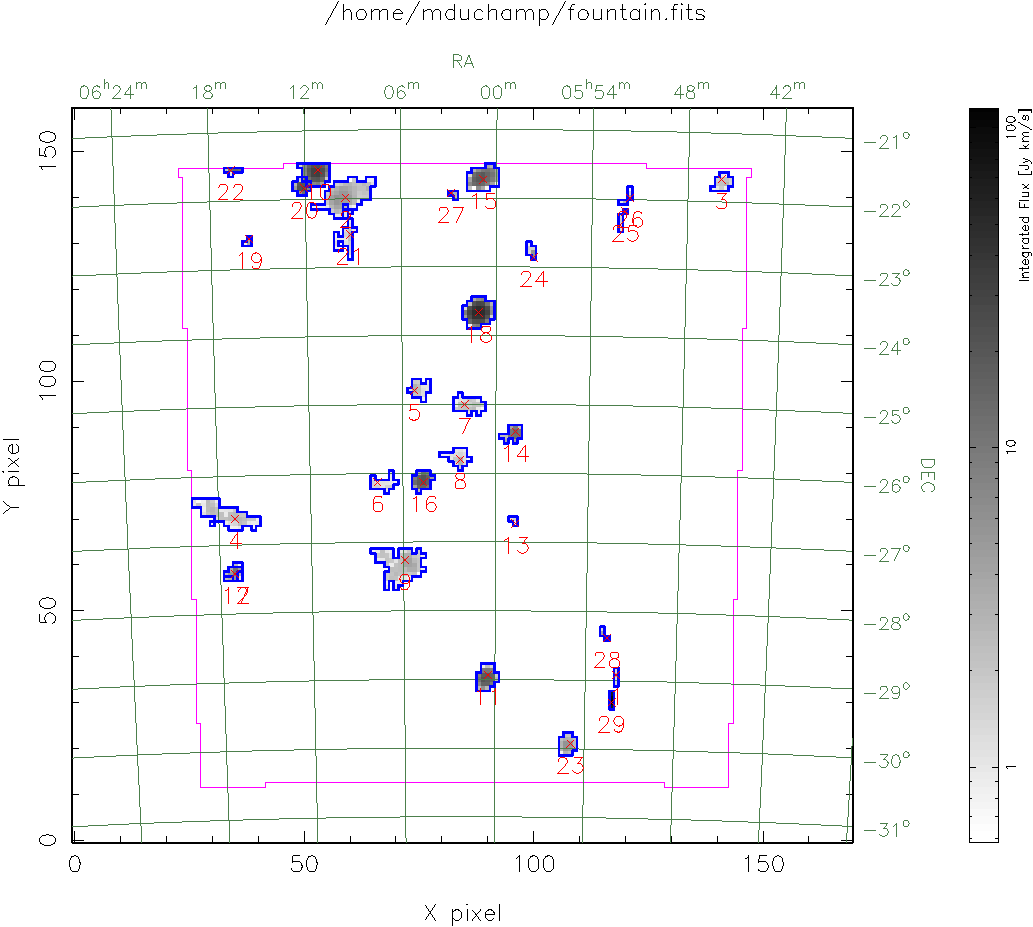
\includegraphics[width=\textwidth]{example_moment_map}
\end{center}
\caption{\footnotesize An example of the moment map created by
  Duchamp. The full extent of the cube is covered, and the 0th moment
  of each object is shown (integrated individually over all the
  detected channels).}
\label{fig-moment}
\end{figure}

As well as the output data file, a postscript file is created that
shows the spectra of each detection, together with a small cutout
image (0th moment) and basic information of the detection. If the cube
was reconstructed, the spectrum from the reconstruction is shown in
red, over the top of the original spectrum. The spectrum that is
plotted is governed by the {\tt spectralMethod} parameter. It can be
either {\tt peak}, where the spectrum is that containing the pixel
with the detection's peak flux; or {\tt sum}, where the spectrum is
summed over all spatial pixels, and then corrected for the beam size.

The spectral extent of the detection is indicated with blue lines, and
a zoom is shown in a separate window. The cutout image can optionally
include a border around the spatial pixels that are in the detection
(turned on and off by the parameter {\tt drawBorders}). It also
includes a scale bar in the bottom left corner to indicate size -- it
is 30~arcmin long. An example detection can be seen below in
Fig.~\ref{fig-spect}.

Finally, a couple of images are optionally produced: a 0th moment map
of the cube, combining just the detected channels in each object,
showing the integrated flux in grey-scale; and a ``detection image'',
a grey-scale image where the pixel values are the number of channels
that spatial pixel is detected in. In both cases, if {\tt drawBorders =
true}, a border is drawn around the spatial extent of each
detection. An example moment map is shown in Fig.~\ref{fig-moment}.
The production or otherwise of these images is governed by the {\tt
flagMaps} parameter.

The purpose of these images are to provide a visual guide to where the
detections have been made, and, particularly in the case of the moment
map, to provide an indication of the strength of the source. In both
cases, the detections are numbered (in the same way as the output
list), and the spatial borders are marked out as for the cutout images
in the spectra file. Both these images are saved as postscript files
(given by the parameters {\tt momentMap} and {\tt detectionMap}
respectively), with the latter also displayed in a {\sc pgplot}
window (regardless of the state of {\tt flagMaps}).

\section{Notes and hints on the use of Duchamp}

In using Duchamp, the user has to make a number of decisions about
the way the program runs. This section is designed to give the user
some idea about what the various selections do...

The main choice is whether or not to use the wavelet
reconstruction. The main benefits of this are the marked reduction in
the noise level, leading to regularly-shaped detections, and good
reliability for faint sources. The main drawback with its use is the
long execution time: to reconstruct a $170\times160\times1024$
(\hipass) cube often requires three iterations and takes about 20-25
minutes. The searching part of the procedure is much quicker (although
see the note on merging, below), so if one uses the FDR method on the
un-reconstructed cube, the execution time is only a couple of minutes.

A further drawback with the reconstruction is that it is susceptible
to edge effects. If the valid area in the cube (\ie the part that is
not BLANK) has very curved edges (such as the \hipass\ polar cap cube,
H001, which has a roughly circular shape after gridding), the
convolution can produce artefacts in the reconstruction that mimic
the edges and lead to some spurious sources. Caution is advised with
such data -- the user is advised to check carefully the reconstructed
cube for the presence of such artefacts.

If one chooses the reconstruction method, a further decision is
required on the signal-to-noise cutoff used in determining acceptable
wavelet coefficients. A larger value will remove more noise from the
cube, at the expense of losing fainter sources, while a smaller value
will include more noise, which may produce spurious detections, but
will be more sensitive to faint sources. Values of less than about
$3\sigma$ tend to not reduce the noise a great deal and can lead to
many spurious sources.

The FDR method certainly produces more reliable results than a simple
sigma-clipping (\ie thresholding at some number of $\sigma$ above the
mean). However, at this point it does not seem to be giving the
sensitivity expected for the supplied value of {\tt alpha} (\ie it is
not finding as many sources as expected). Work is
being done to assess this, and to judge whether there is a real
problem (such as with the determination of the statistics), or simply
a result of working in 3 dimensions as opposed to 2.

A further point to bear in mind is that the shape of the detections in
a cube that has been reconstructed will be much more regular and
smooth -- the ragged edges that objects in the raw cube possess are
smoothed by the removal of most of the noise.

Finally, as Duchamp is still undergoing development, there are some
elements that are not fully developed. In particular, it is not as
clever as I would like at avoiding interference. The ability to place
requirements on the minimum number of channels and pixels partially
circumvents this problem, but work is being done to make Duchamp
smarter at rejecting signals that are clearly (to a human eye at
least) interference. See the following section for further
improvements that are planned.

%\section{Drawbacks of the current program}
%
%The program currently has a few problems/drawbacks/things to be aware
%of that will hopefully be fixed in the future:
%\begin{itemize}
%
%\item Narrow interference spikes are still getting found, particularly
%  if there is no reconstruction, or reconstruction with a relatively
%  low {\tt snrRecon} (such as 2 or 3). Increasing the {\tt
%  minChannels} parameter is one way to circumvent this, but making the
%  algorithm a bit more clever would be preferable.
%
%\item Sources that have strong continuum ripple and/or artefacts often
%  generate many spurious detections. This needs some work to avoid
%  Duchamp doing this, and until then users are advised to be aware
%  of the possibility. Strong continuum ripples may generate many
%  sources on the same spatial pixel, and this will be apparent on the
%  detection images.
%
%\item Spectra are integrated over every spatial pixel of the
%  detection, and this may dilute the actual detection, making it
%  harder to see \ie the apparent strength of the line as plotted may
%  not give a true indication of how strong it really is.
%
%%\item A caution on the merging part of the procedure. This can be time
%%  consuming if there are many detections that do not require merging
%%  -- in this case, the time will go like $N^2$ ($N$ = number of
%%  detections). If there are plenty of mergers, the size of the list
%%  reduces quickly, so the execution time will be less.
%
%
%\end{itemize}


%\section{Comparison with other software (to be developed further...)}
%
%\subsection{fred, by Matt Howlett}
%
%This is the program used in the \hipass\ analysis. It smoothes the
%data spectrally with a boxcar filter of a size that varies over a
%user-specified range, and then thresholds the data.
%
%Works effectively, but generally doesn't find as many sources as
%Duchamp, particularly when the reconstruction is used. Sensitive to
%faint, broad features that fall below the reconstruction threshold.
%
%Execution takes a long time, depending on the range of filter widths
%that are used.
%
%\subsection{sfind}
%
%Hard to evaluate, as it does not (as far as I can see) output the
%channel number at which detections are made, and does not merge
%detections made at adjacent channels (\ie it just works in 2
%dimensions). 
%

\section{Future Developments}

This is both a list of planned improvements and a wish-list of
features that would be nice to include (but are not planned in the
immediate future):

\begin{itemize}

\item Ability to invert cube to search for absorption features. {\bf
  Planned.} 

\item More varied output formats. {\bf Planned.}

\item Better determination of the noise characteristics of
  spectral-line cubes, including understanding how the noise is
  generated and developing a model for it. {\bf Planned.}
  
\item Include more source analysis. Examples could be: shape
  information; measurements of HI mass; better measurements of
  velocity width and profile... {\bf Some planned.}

\item Provide some indication of the significance of the detection
  (\ie some S/N-like value). {\bf Planned.}

\item Improved ability to reject interference, possibly on the
  spectral shape of features. {\bf Planned.}

\item Link to lists of possible counterparts (\eg via NED/SIMBAD/other
  VO tools?). {\bf Wishlist.} 

\item Add ability to read in a reconstructed cube that has been
  saved. In this case the residual array will also need to be read
  in. The idea of this will be to avoid the extended time required for
  the reconstruction if the same cube is being analysed multiple
  times. {\bf Wishlist.}
 
\item At this point, the ``Milky Way'' channels are discarded and set
  to zero. It may be that users would like to have those put back in
  the final cube after the source detection is done, so at some point
  this option may be added. {\bf Wishlist -- if needed.}

\end{itemize}


%\bibliographystyle{mn2e}
%\bibliographystyle{abbrvnat}
%\bibliography{mnrasmnemonic,sourceDetection}
\begin{thebibliography}{}

\bibitem[\protect\citeauthoryear{{Calabretta} \& {Greisen}}{{Calabretta} \&
  {Greisen}}{2002}]{calabretta02}
{Calabretta} M.,  {Greisen} E.,  2002, A\&A, 395, 1077

\bibitem[\protect\citeauthoryear{{Greisen} \& {Calabretta}}{{Greisen} \&
  {Calabretta}}{2002}]{greisen02}
{Greisen} E.,  {Calabretta} M.,  2002, A\&A, 395, 1061

\bibitem[\protect\citeauthoryear{{Hanisch}, {Farris}, {Greisen}, {Pence},
  {Schlesinger}, {Teuben}, {Thompson} \& {Warnock}}{{Hanisch}
  et~al.}{2001}]{hanisch01}
{Hanisch} R.,  {Farris} A.,  {Greisen} E.,  {Pence} W.,  {Schlesinger} B.,
  {Teuben} P.,  {Thompson} R.,    {Warnock} A.,  2001, A\&A, 376, 359

\bibitem[\protect\citeauthoryear{{Hopkins}, {Miller}, {Connolly}, {Genovese},
  {Nichol} \& {Wasserman}}{{Hopkins} et~al.}{2002}]{hopkins02}
{Hopkins} A.,  {Miller} C.,  {Connolly} A.,  {Genovese} C.,  {Nichol} R.,
  {Wasserman} L.,  2002, AJ, 123, 1086

\bibitem[\protect\citeauthoryear{Lutz}{Lutz}{1980}]{lutz80}
Lutz R.,  1980, The Computer Journal, 23, 262

\bibitem[\protect\citeauthoryear{{Meyer} et~al.,}{{Meyer}
  et~al.}{2004}]{meyer04:trunc}
{Meyer} M.,  et~al., 2004, MNRAS, 350, 1195

\bibitem[\protect\citeauthoryear{{Miller}, {Genovese}, {Nichol}, {Wasserman},
  {Connolly}, {Reichart}, {Hopkins}, {Schneider} \& {Moore}}{{Miller}
  et~al.}{2001}]{miller01}
{Miller} C.,  {Genovese} C.,  {Nichol} R.,  {Wasserman} L.,  {Connolly} A.,
  {Reichart} D.,  {Hopkins} A.,  {Schneider} J.,    {Moore} A.,  2001, AJ, 122,
  3492

\bibitem[\protect\citeauthoryear{Minchin}{Minchin}{1999}]{minchin99}
Minchin R.,  1999, PASA, 16, 12

\bibitem[\protect\citeauthoryear{Starck \& Murtagh}{Starck \&
  Murtagh}{2002}]{starck02:book}
Starck J.-L.,  Murtagh F.,  2002, {``Astronomical Image and Data Analysis''}.
Springer

\end{thebibliography}


\appendix
\newpage
\section{Available parameters}
\label{app-param}

The full list of parameters that can be listed in the input file are
given here. If not listed, they take the default value given in
parentheses. Since the order of the parameters in the input file does
not matter, they are grouped here in logical sections.

\subsection*{Input-output related}
\begin{entry}
\item[ImageFile (no default assumed)] The filename of the
  data cube to be analysed.
\item[OutFile {\tt [./duchamp-Results]}] The file where the final
  detections are to be recorded. This also records the list of input
  parameters.
\item[SpectraFile {\tt [./duchamp-Spectra.ps]}] The postscript file
  containing the resulting integrated spectra and images of the
  detections. 
\item[flagLog {\tt [true]}] A flag to indicate whether intermediate
  detections should be logged.
\item[LogFile {\tt [./duchamp-Logfile]}] The file in which intermediate
  detections are logged. These are detections that have not been
  merged. This is primarily for use in debugging and diagnostic
  purposes -- normal use of the program will probably not require
  this.
\item[flagSubsection {\tt [false]}] A flag to indicate whether one
  wants a subsection of the requested image.
\item[Subsection {\tt [ [*,*,*] ]}] The requested subsection, which
  should be specified in the format {\tt [x1:x2,y1:y2,z1:z2]}, where
  the limits are inclusive. If the full range of a dimension is
  required, use a {\tt *}, \eg if you want the full spectral range of
  a subsection of the image, use {\tt [30:140,30:140,*]}.
\item[flagOutputRecon {\tt [false]}] A flag to say whether or not to
  save the reconstructed cube as a FITS file. The filename will be
  derived from the ImageFile -- the reconstruction of {\tt image.fits}
  will be saved as {\tt image.RECON?.fits}, where {\tt ?} stands for
  the value of {\tt snrRecon} (see below).
\item[flagOutputResid {\tt [false]}] As for {\tt flagOutputRecon}, but
  for the residual array -- the difference between the original cube
  and the reconstructed cube. The filename will be {\tt
  image.RESID?.fits}.
\item[flagVOT {\tt [false]}] A flag to say whether to create a VOTable
  file corresponding to the information in {\tt outfile}. This will be
  an XML file in the Virtual Observatory VOTable format.
\item[votFile {\tt [./duchamp-Results.xml]}] The VOTable file with the
  list of final detections. Some input parameters are also recorded.
\item[flagKarma {\tt [false]}] A flag to say whether to create a Karma
  annotation file corresponding to the information in {\tt
  outfile}. This can be used as an overlay for the Karma programs such
  as {\tt kvis}.
\item[karmaFile {\tt [./duchamp-Results.ann]}] The Karma annotation
  file showing the list of final detections. 
\item[flagMaps {\tt [true]}] A flag to say whether to save postscript
  files showing the 0th moment map of the whole cube (parameter {\tt
  momentMap}) and the detection image ({\tt detectionMap}).
\item[momentMap {\tt [./latest-moment-map.ps]}] A postscript file
  containing a map of the 0th moment of the detected sources, as well
  as pixel and WCS coordinates.
\item[detectionMap {\tt [./latest-detection-map.ps]}] A postscript
  file showing each of the detected objects, coloured in greyscale by
  the number of channels they span. Also shows pixel and WCS
  coordinates.
\end{entry}

\subsection*{Modifying the cube}
\begin{entry}
\item[flagBlankPix {\tt [true]}] A flag to say whether to remove BLANK
  pixels from the analysis -- these are pixels set to some particular
  value because they fall outside the imaged area.
\item[blankPixValue {\tt [-8.00061]}] The value of the BLANK pixels,
  if this information is not contained in the FITS header (the usual
  procedure is to obtain this value from the header information -- in
  which case the value set by this parameter is ignored).
\item[flagMW {\tt [false]}] A flag to say whether to remove channels
  contaminated by Milky Way (or other) emission -- the flux in these
  channels is currently just set to 0.
\item[maxMW {\tt [112]}] The maximum channel for the Milky Way
  emission.
\item[minMW {\tt [75]}] The minimum channel for the Milky Way
  emission. Note that the channels specified by {\tt maxMW} and {\tt
  minMW} are assumed to be Milky Way channels (\ie the range is
  inclusive).
\item[flagBaseline {\tt [false]}] A flag to say whether to remove the
  baseline from each spectrum in the cube for the purposes of
  reconstruction and detection.
\end{entry}

\subsection*{Detection related}

\subsubsection*{General detection}
\begin{entry}
\item[snrCut {\tt [3.]}] The cut-off value for thresholding, in terms
  of number of $\sigma$ above the mean.
\item[flagGrowth {\tt [true]}] A flag indicating whether or not to
  grow the detected objects to a smaller threshold.
\item[growthCut {\tt [1.5]}] The smaller threshold using in growing
  detections. In units of $\sigma$ above the mean.
\end{entry}

\subsubsection*{{\` a} trous reconstruction}
\begin{entry}
\item [flagATrous {\tt [true]}] A flag indicating whether or not to
  reconstruct the cube using the {\it {\`a} trous} wavelet
  reconstruction. Currently does this in 3-dimensions. See
  \S\ref{sec-recon} for details.
\item[scaleMin {\tt [1]}] The minimum wavelet scale to be used in the
  reconstruction. A value of 1 means ``use all scales''.
\item[snrRecon {\tt [4]}] The thresholding cutoff used in the
  reconstruction -- only wavelet coefficients this many $\sigma$ above
  the mean (or greater) are included in the reconstruction. 
\item[filterCode {\tt [2]}] The code number of the filter to use in
  the reconstruction. The options are:
  \begin{itemize}
  \item {\bf 1:} B$_3$-spline filter: coefficients = 
    $(\frac{1}{16}, \frac{1}{4}, \frac{3}{8}, \frac{1}{4}, \frac{1}{16})$
  \item {\bf 2:} Triangle filter: coefficients = $(\frac{1}{4}, \frac{1}{2}, \frac{1}{4})$
  \item {\bf 3:} Haar wavelet: coefficients = $(0, \frac{1}{2}, \frac{1}{2})$
  \end{itemize}
\end{entry}

\subsubsection*{FDR method}
\begin{entry}
\item[flagFDR {\tt [false]}] A flag indicating whether or not to use
  the False Discovery Rate method in thresholding the pixels.
\item[alphaFDR {\tt [0.01]}] The $\alpha$ parameter used in the FDR
analysis. The average number of false detections, as a fraction of the
total number, will be less than $\alpha$ (see \S\ref{sec-detection}).
\end{entry}

\subsubsection*{Merging detections}
\begin{entry}
\item[flagAdjacent {\tt [true]}] A flag indicating whether to use the
  ``adjacent pixel'' criterion to decide whether to merge objects. If
  not, the next two parameters are used to determine whether objects
  are within the necessary thresholds.
\item[minPix {\tt [2]}] The minimum number of spatial pixels for a single
  detection to be counted.
\item[minChannels {\tt [3]}] The minimum number of consecutive
  channels that must be present in the detection for it to be accepted
  by the Merging algorithm.
%The minimum number of channels that a
%  detection must span for it to be accepted by the Merging algorithm.
\item[threshSpatial {\tt [3.]}] The maximum allowed minimum spatial
  separation (in pixels) between two detections for them to be merged
  into one. Only used if {\tt flagAdjacent = false}.
\item[threshVelocity {\tt [7.]}] The maximum allowed minimum channel
  separation between two detections for them to be merged into
  one. %Only used if {\tt flagAdjacent = false}.
\end{entry}

\subsubsection*{Other parameters}
\begin{entry}
\item[spectralMethod {\tt [peak]}] This indicates which method to plot
  the output spectra by: {\tt peak} means plot the spectrum containing
  the detection's peak pixel; {\tt sum} means sum the spectra of each
  detected spatial pixel, and correct for the beam size. Any other
  choice defaults to {\tt peak}.
\item[drawBorders {\tt [true]}] A flag indicating whether borders
  are to be drawn around the detected objects in the moment maps
  included in the output (see for example Fig.~\ref{fig-spect}).
\item[verbose {\tt [true]}] A flag indicating whether to print the
  progress of computationally-intensive algorithms (such as the
  searching and merging) to screen.
\end{entry}


\newpage
\section{Example parameter files}
\label{app-input}

This is what a typical parameter file would look like.

\begin{verbatim}
imageFile       /DATA/SITAR_1/whi550/cubes/H201_abcde_luther_chop.fits
logFile         temp-Logfile
outFile         temp-Results
spectraFile     spectra.ps
flagSubsection  0
flagOutputRecon 0
flagOutputResid 0
flagBlankPix    1
blankPixValue   -8.00061
flagMW          1
minMW           75
maxMW           112
minPix          3
flagGrowth      1
growthCut       1.5
flagATrous      0
scaleMin        1
snrRecon        4
flagFDR         1
alphaFDR        0.1
numPixPSF       20
snrCut          3
threshSpatial   3
threshVelocity  7
minChannels     4
\end{verbatim}

Note that it is not necessary to include all these parameters in the
file, only those that need to be changed from the defaults (as listed
in Appendix~\ref{app-param}), which in this case would be very few. A
minimal parameter file might look like:
\begin{verbatim}
imageFile       /DATA/SITAR_1/whi550/cubes/H201_abcde_luther_chop.fits
flagLog         0
snrRecon        3
snrCut          2.5
minChannels     3
\end{verbatim}
This will reconstruct the cube with a lower SNR value than the
default, select objects at a lower threshold,  with a looser minimum
channel requirement, and not keep a log of the intermediate
detections. 

The following page demonstrates how the parameters are presented to
the user, both on the screen at execution time and in the output and
log files:
\newpage
\begin{landscape}
Presentation of parameters in output and log files:  
\begin{verbatim}
---- Parameters ----
Image to be analysed                    = /DATA/SITAR_1/whi550/cubes/H201_abcde_luther_chop.fits
Intermediate Logfile                    = logfile.txt
Final Results file                      = results.txt
Spectrum file                           = spectra.ps
VOTable file                            = results.xml
0th Moment Map                          = latest-moment-map.ps
Detection Map                           = latest-detection-map.ps
Saving reconstructed cube?              = false
Saving residuals from reconstruction?   = false
------
Fixing Blank Pixels?                    = true
Blank Pixel Value                       = -8.00061
Removing Milky Way channels?            = true
Milky Way Channels                      = 75-112
Beam Size (pixels)                      = 10.1788
Removing baselines before search?       = false
Minimum # Pixels in a detection         = 2
Growing objects after detection?        = false
Using A Trous reconstruction?           = true
Minimum scale in reconstruction         = 1
SNR Threshold within reconstruction     = 4
Filter being used for reconstruction    = B3 spline function
Using FDR analysis?                     = false
SNR Threshold                           = 2.5
Using Adjacent-pixel criterion?         = true
Min. # channels for merging             = 4
--------------------
\end{verbatim}

\newpage
\section{Example output file}
\label{app-output}
This the typical content of an output file, after running Duchamp
with the parameters illustrated on the previous page.

{\scriptsize 
  \begin{verbatim}
Results of the Duchamp source finder: Tue Mar 21 16:28:50 EST 2006
---- Parameters ----

(... omitted for clarity -- see previous page for examples...)

--------------------
Total number of detections = 23
--------------------
 Obj#          Name     X     Y      Z           RA          DEC    w_RA   w_DEC       VEL    w_VEL  X1  X2  Y1  Y2   Z1   Z2  Npix     F_tot  F_peak
-----------------------------------------------------------------------------------------------------------------------------------------------------
    1    J0609-2200  59.4 140.6  114.7  06:09:38.50 -22:00:48.20   48.50   39.42   213.061   65.957  55  66 136 145  113  118   185   17.5725  0.2125
    2    J0608-2605  65.2  79.6  116.2  06:08:10.23 -26:05:06.57   44.47   39.47   233.119   39.574  60  70  76  85  115  118    50    4.1441  0.1002
    3    J0606-2724  70.8  59.8  121.4  06:06:33.08 -27:24:43.28   52.48   47.57   302.213   39.574  65  77  53  64  120  123   213   17.0659  0.1497
    4    J0611-2142  52.5 145.1  162.5  06:11:36.34 -21:42:00.01   32.40   23.47   843.727  118.722  49  56 142 147  158  167   303   44.3940  0.4103
    5    J0600-2903  89.7  35.3  202.4  06:00:51.38 -29:03:02.51   23.94   28.09  1370.285  184.679  87  92  32  38  195  209   319   26.5725  0.1729
    6    J0559-2643  95.5  70.2  222.6  05:59:10.59 -26:43:05.94   15.94   12.09  1637.316  105.531  94  97  69  71  219  227    35    1.9253  0.0630
    7    J0617-2727  34.8  58.3  227.5  06:17:24.45 -27:27:53.89   20.77   23.41  1701.802  303.400  33  37  56  61  215  238   176   11.4138  0.0929
    8    J0609-2145  60.3 144.4  229.6  06:09:23.17 -21:45:36.06   16.15   11.81  1729.279  105.531  59  62 143 145  225  233    25    1.4760  0.0679
    9    J0559-2529  95.7  88.6  231.1  05:59:08.81 -25:29:34.50   27.88   24.14  1749.440  250.635  92  98  86  91  220  239   257   16.9297  0.1155
   10    J0601-2145  88.9 144.4  232.3  06:01:10.14 -21:45:58.59   31.96   24.13  1764.657  224.253  86  93 142 147  222  239   415   34.0304  0.1655
   11    J0615-2638  40.0  70.8  232.6  06:15:44.32 -26:38:29.42   16.56   19.57  1769.033   52.765  38  41  69  73  231  235    44    2.7565  0.0685
   12    J0605-2610  75.9  78.4  233.1  06:05:00.16 -26:10:21.68   28.14   23.84  1775.066  224.253  73  79  76  81  225  242   352   27.0587  0.1545
   13    J0601-2344  88.0 114.9  235.7  06:01:25.72 -23:44:18.18   35.96   32.07  1809.749  263.826  84  92 112 119  226  246   724   85.1317  0.2968
   14    J0615-2238  38.2 130.6  253.6  06:15:48.32 -22:38:45.75   12.39   15.70  2046.530  118.722  37  39 129 132  248  257    40    2.3169  0.0697
   15    J0617-2309  31.4 122.8  258.0  06:17:51.07 -23:09:29.22   16.46   15.53  2103.912   39.574  30  33 121 124  256  259    23    1.4243  0.0624
   16    J0612-2153  49.5 142.3  271.1  06:12:29.32 -21:53:16.05   24.36   19.56  2276.976  395.740  47  52 140 144  257  287   318   20.7117  0.1008
   17    J0616-2137  35.2 145.9  300.0  06:16:34.07 -21:37:30.95   20.22    7.46  2658.607  224.252  33  37 145 146  294  311    40    3.8507  0.1271
   18    J0544-2740 144.0  54.9  325.4  05:44:31.07 -27:40:42.30    3.58   12.13  2993.384   39.574 144 144  54  56  324  327     7    0.4362  0.0569
   19    J0555-3000 107.2  20.7  367.5  05:55:28.58 -30:00:46.76   19.67   24.31  3547.812   39.574 105 109  18  23  366  369    72    6.4819  0.1692
   20    J0559-2325  96.0 119.6  532.1  05:59:04.98 -23:25:19.04   11.92   16.08  5720.289   52.765  95  97 118 121  530  534    27    1.2865  0.0508
   21    J0616-2653  37.9  67.0  547.0  06:16:23.08 -26:53:11.73   12.36   11.67  5916.731   39.574  37  39  66  68  546  549    25    1.6374  0.0642
   22    J0619-2256  25.1 125.9  724.2  06:19:39.49 -22:56:06.15   12.38   11.60  8254.112   39.573  24  26 125 127  723  726    13    0.6982  0.0593
   23    J0552-2920 116.9  30.5  727.0  05:52:33.03 -29:20:54.43   11.60   20.25  8290.842  303.400 116 118  28  32  716  739   132   35.8343  0.4787
  \end{verbatim}
}

%\end{landscape}

\newpage
\section{Example VOTable output}
\label{app-votable}
This is part of the VOTable, in XML format, corresponding to the
output file in Appendix~\ref{app-output} (the indentation has been removed to make it fit on the page!).

%\begin{landscape}
{\scriptsize
  \begin{verbatim}
<?xml version="1.0"?>
<VOTABLE version="1.1" xmlns:xsi="http://www.w3.org/2001/XMLSchema-instance"
 xsi:noNamespaceSchemaLocation="http://www.ivoa.net/xml/VOTable/VOTable/v1.1">
<COOSYS ID="J2000" equinox="J2000." epoch="J2000." system="eq_FK5"/>
<RESOURCE name="Duchamp Output">
<TABLE name="Detections">
<DESCRIPTION>Detected sources and parameters from running the Duchamp source finder.</DESCRIPTION>
<PARAM name="FITS file" datatype="char" ucd="meta.file;meta.fits" value="/DATA/SITAR_1/whi550/cubes/H201_abcde_luther_chop.fits"/>
<FIELD name="ID" ID="col1" ucd="meta.id" datatype="int" width="4"/>
<FIELD name="Name" ID="col2" ucd="meta.id;meta.main" datatype="char" arraysize="14"/>
<FIELD name="RA" ID="col3" ucd="pos.eq.ra;meta.main" ref="J2000" datatype="float" width="10" precision="6" unit="deg"/>
<FIELD name="Dec" ID="col4" ucd="pos.eq.dec;meta.main" ref="J2000" datatype="float" width="10" precision="6" unit="deg"/>
<FIELD name="w_RA" ID="col3" ucd="phys.angSize;pos.eq.ra" ref="J2000" datatype="float" width="7" precision="2" unit="arcmin"/>
<FIELD name="w_Dec" ID="col4" ucd="phys.angSize;pos.eq.dec" ref="J2000" datatype="float" width="7" precision="2" unit="arcmin"/>
<FIELD name="Vel" ID="col4" ucd="phys.veloc;src.dopplerVeloc" datatype="float" width="9" precision="3" unit="km/s"/>
<FIELD name="w_Vel" ID="col4" ucd="phys.veloc;src.dopplerVeloc;spect.line.width" datatype="float" width="8" precision="3" unit="km/s"/>
<FIELD name="Integrated_Flux" ID="col4" ucd="phys.flux;spect.line.intensity" datatype="float" width="10" precision="3" unit="km/s"/>
<DATA>
<TABLEDATA>
<TR>
<TD>   1</TD><TD>    J0609-2200</TD><TD> 92.410416</TD><TD>-22.013390</TD><TD>  48.50</TD><TD>  39.42</TD><TD>  213.061</TD><TD>  65.957</TD><TD>    17.572</TD>
</TR>
<TR>
<TD>   2</TD><TD>    J0608-2605</TD><TD> 92.042633</TD><TD>-26.085157</TD><TD>  44.47</TD><TD>  39.47</TD><TD>  233.119</TD><TD>  39.574</TD><TD>     4.144</TD>
</TR>
<TR>
<TD>   3</TD><TD>    J0606-2724</TD><TD> 91.637840</TD><TD>-27.412022</TD><TD>  52.48</TD><TD>  47.57</TD><TD>  302.213</TD><TD>  39.574</TD><TD>    17.066</TD>
</TR>
<TR>
<TD>   4</TD><TD>    J0611-2142</TD><TD> 92.901421</TD><TD>-21.700003</TD><TD>  32.40</TD><TD>  23.47</TD><TD>  843.727</TD><TD> 118.722</TD><TD>    44.394</TD>
</TR>
<TR>
<TD>   5</TD><TD>    J0600-2903</TD><TD> 90.214081</TD><TD>-29.050697</TD><TD>  23.94</TD><TD>  28.09</TD><TD> 1370.285</TD><TD> 184.679</TD><TD>    26.573</TD>
</TR>
(... table truncated for clarity ...)
</TABLEDATA>
</DATA>
</TABLE>
</RESOURCE>
</VOTABLE>
  \end{verbatim}
}
\end{landscape}

\section{Robust statistics for a Normal distribution}
\label{app-madfm}

The Normal, or Gaussian, distribution for mean $\mu$ and standard
deviation $\sigma$ can be written as 
\[ 
f(x) = \frac{1}{\sqrt{2\pi\sigma^2}}\ e^{-(x-\mu)^2/2\sigma^2}.
 \]

When one has a purely Gaussian signal, it is straightforward to
estimate $\sigma$ by calculating the standard deviation (or rms) of
the data. However, if there is a small amount of signal present on top
of Gaussian noise, and one wants to estimate the $\sigma$ for the
noise, the presence of the large values from the signal can bias the
estimator to higher values.

An alternative way is to use the median ($m$) and median absolute deviation
from the median ($s$) to estimate $\mu$ and $\sigma$. The median is the
middle of the distribution, defined for a continuous distribution by
\[
\int_{-\infty}^{m} f(x) \diff x = \int_{m}^{\infty} f(x) \diff x.
\]
From symmetry, we quickly see that for the continuous Normal
distribution, $m=\mu$. We consider the case henceforth of $\mu=0$,
without loss of generality.

To find $s$, we find the distribution of the absolute deviation from
the median, and then find the median of that distribution. This
distribution is given by
\begin{eqnarray*}
g(x) &= &{\mbox{\rm distribution of }} |x|\\
     &= &f(x) + f(-x),\ x\ge0\\
     &= &\sqrt{\frac{2}{\pi\sigma^2}}\, e^{-x^2/2\sigma^2},\ x\ge0.
\end{eqnarray*}
So, the median absolute deviation from the median, $s$, is given by
\[
\int_{0}^{s} g(x) \diff x = \int_{s}^{\infty} g(x) \diff x.
\]
Now, $\int_{0}^{\infty}e^{-x^2/2\sigma^2} \diff x = \sqrt{\pi\sigma^2/2}$, and
so $\int_{s}^{\infty} e^{-x^2/2\sigma^2} \diff x =
\sqrt{\pi\sigma^2/2} - \int_{0}^{s} e^{-\frac{x^2}{2\sigma^2}} \diff x
$. Hence, to find $s$ we simply solve the following equation (setting $\sigma=1$ for
simplicity -- equivalent to stating $x$ and $s$ in units of $\sigma$):
\[
\int_{0}^{s}e^{-x^2/2} \diff x - \sqrt{\pi/8} = 0.
\]
This is hard to solve analytically (no nice analytic solution exists
for the finite integral that I'm aware of), but straightforward to
solve numerically, yielding the value of $s=0.6744888$. Thus, to
estimate $\sigma$ for a Normally distributed data set, one can calculate
$s$, then divide by 0.6744888 (or multiply by 1.4826042) to obtain the
correct estimator.

Note that this is different to solutions quoted elsewhere,
specifically in \citet{meyer04:trunc}, where the same robust estimator
is used but with an incorrect conversion to standard deviation -- they
assume $\sigma = s\sqrt{\pi/2}$. This, in fact, is the conversion used
to convert the {\it mean} absolute deviation from the mean to the
standard deviation. This means that the cube noise in the \hipass\
catalogue (parameter Rms$_{\rm cube}$) should be 18\% larger than
quoted.

%a different value for $s/\sigma$ (of
%$\sqrt{2/\pi}\approx0.797885$) is quoted. It should thus be noted that
%this means the values quoted by \citet{meyer04:trunc} for the cube noise in
%the \hipass\ catalogue should be 18\% larger (since 0.1486042 is 18\%
%larger than $\sqrt{\pi/2}\approx1.253314$). 

\section{How Gaussian noise changes with wavelet scale.}
\label{app-scaling}

The key element in the wavelet reconstruction of an array is the
thresholding of the individual wavelet coefficient arrays. This is
usually done by choosing a level to be some number of standard
deviations above the mean value.

However, since the wavelet arrays are produced by convolving the input
array by an increasingly large filter, the pixels in the coefficient
arrays become increasingly correlated as the scale of the filter
increases. This results in the measured standard deviation from a
given coefficient array decreasing with increasing scale. To calculate
this, we need to take into account how many other pixels each pixel in
the convolved array depends on.

To demonstrate, suppose we have a 1-D array with $N$ pixel values
given by $F_i,\ i=1,...,N$, and we convolve it with the B$_3$-spline
filter with coefficients $\{1/16,1/4,3/8,1/4,1/16\}$. The flux of the
$i$th pixel in the convolved array will be
\[
F'_i = \frac{1}{16}F_{i-2} + \frac{1}{16}F_{i-2} + \frac{3}{8}F_{i}
+ \frac{1}{4}F_{i-1} + \frac{1}{16}F_{i+2}
\]
and the flux of the corresponding pixel in the wavelet array will be 
\[
W'_i = F_i - F'_i = \frac{1}{16}F_{i-2} + \frac{1}{16}F_{i-2} + \frac{5}{8}F_{i}
+ \frac{1}{4}F_{i-1} + \frac{1}{16}F_{i+2}
\]
Now, assuming each pixel has the same standard deviation
$\sigma_i=\sigma$, we can work out the standard deviation for the
coefficient array:
\[
\sigma'_i = \sigma \sqrt{\left(\frac{1}{16}\right)^2 + \left(\frac{1}{4}\right)^2
  + \left(\frac{5}{8}\right)^2 + \left(\frac{1}{4}\right)^2 + \left(\frac{1}{16}\right)^2}
          = 0.72349\ \sigma
\]
Thus, the first scale wavelet coefficient array will have a standard
deviation of 72.3\% of the input array. This procedure can be followed
to calculate the necessary values for all scales, dimensions and
filters used by Duchamp.

Calculating these values is, therefore, a critical step in performing
the reconstruction. \citet{starck02:book} did so by simulating data sets
with Gaussian noise, taking the wavelet transform, and measuring the
value of $\sigma$ for each scale. We take a different approach, by
calculating the scaling factors directly from the filter coefficients
by taking the wavelet transform of an array made up of a 1 in the
central pixel and 0s everywhere else. The scaling value is then
derived by adding in quadrature all the wavelet coefficient values at
each scale. We give the scaling factors for the three filters
available to Duchamp on the following page. These values are
hard-coded into Duchamp, so no on-the-fly calculation of them is
necessary. 

Memory limitations prevent us from calculating factors for large
scales, particularly for the three-dimensional case (hence the --
symbols in the tables). To calculate factors for
higher scales than those available, we note the following
relationships apply for large scales to a sufficient level of precision:
\begin{itemize}
\item 1-D: factor(scale $i$) = factor(scale $i-1$)$/\sqrt{2}$.
\item 2-D: factor(scale $i$) = factor(scale $i-1$)$/2$.
\item 1-D: factor(scale $i$) = factor(scale $i-1$)$/\sqrt{8}$.
\end{itemize}

\newpage
\begin{itemize}
\item {\bf B$_3$-Spline Function:} $\{1/16,1/4,3/8,1/4,1/16\}$

\begin{tabular}{llll}
Scale & 1 dimension      & 2 dimension     & 3 dimension\\ \hline
1     & 0.723489806      & 0.890796310     & 0.956543592\\
2     & 0.285450405	 & 0.200663851	   & 0.120336499\\
3     & 0.177947535	 & 0.0855075048	   & 0.0349500154\\
4     & 0.122223156	 & 0.0412474444	   & 0.0118164242\\
5     & 0.0858113122	 & 0.0204249666	   & 0.00413233507\\
6     & 0.0605703043	 & 0.0101897592	   & 0.00145703714\\
7     & 0.0428107206	 & 0.00509204670   & 0.000514791120\\
8     & 0.0302684024	 & 0.00254566946   & --\\
9     & 0.0214024008	 & 0.00127279050   & --\\
10    & 0.0151336781	 & 0.000636389722  & --\\
11    & 0.0107011079	 & 0.000318194170  & --\\
12    & 0.00756682272	 & --		   & --\\
13    & 0.00535055108	 & --		   & --\\
%14    & 0.00378341085	 & --		   & --\\
%15    & 0.00267527545	 & --		   & --\\
%16    & 0.00189170541	 & --		   & --\\
%17    & 0.00133763772	 & --		   & --\\
%18    & 0.000945852704   & --		   & --
\end{tabular}

\item {\bf Triangle Function:} $\{1/4,1/2,1/4\}$

\begin{tabular}{llll}
Scale & 1 dimension      & 2 dimension     & 3 dimension\\ \hline
1     & 0.612372436      & 0.800390530     & 0.895954449  \\
2     & 0.330718914	 & 0.272878894     & 0.192033014\\
3     & 0.211947812	 & 0.119779282     & 0.0576484078\\
4     & 0.145740298	 & 0.0577664785    & 0.0194912393\\
5     & 0.102310944	 & 0.0286163283    & 0.00681278387\\
6     & 0.0722128185	 & 0.0142747506    & 0.00240175885\\
7     & 0.0510388224	 & 0.00713319703   & 0.000848538128 \\
8     & 0.0360857673	 & 0.00356607618   & 0.000299949455 \\
9     & 0.0255157615	 & 0.00178297280   & -- \\
10    & 0.0180422389	 & 0.000891478237  & --  \\
11    & 0.0127577667	 & 0.000445738098  & --  \\
12    & 0.00902109930	 & 0.000222868922  & --  \\
13    & 0.00637887978	 & --		   & -- \\
%14   & 0.00451054902	 & --		   & -- \\
%15   & 0.00318942978	 & --		   & -- \\
%16   & 0.00225527449	 & --		   & -- \\
%17   & 0.00159471988	 & --		   & -- \\
%18   & 0.000112763724	 & --		   & -- 

\end{tabular}

\item {\bf Haar Wavelet:} $\{0,1/2,1/2\}$

\begin{tabular}{llll}
Scale & 1 dimension      & 2 dimension     & 3 dimension\\ \hline
1     & 0.707167810      & 0.433012702     & 0.935414347 \\
2     & 0.500000000	 & 0.216506351     & 0.330718914\\
3     & 0.353553391	 & 0.108253175     & 0.116926793\\
4     & 0.250000000	 & 0.0541265877    & 0.0413398642\\
5     & 0.176776695	 & 0.0270632939    & 0.0146158492\\
6     & 0.125000000	 & 0.0135316469    & 0.00516748303

\end{tabular}


\end{itemize}

\end{document}

































